\documentclass{beamer}
%
% Choose how your presentation looks.
%
% For more themes, color themes and font themes, see:
% http://deic.uab.es/~iblanes/beamer_gallery/index_by_theme.html
%
\mode<presentation>
{
  \usetheme{Madrid}      % or try Darmstadt, Madrid, Warsaw, ...
  \usecolortheme{beaver} % or try albatross, beaver, crane, ...
  \usefonttheme{serif}  % or try serif, structurebold, ...
  \setbeamertemplate{navigation symbols}{}
  \setbeamertemplate{caption}[numbered]
  \setbeamerfont{frame}{size=\tiny}
} 

\usepackage[english]{babel}
\usepackage[utf8x]{inputenc}
\usepackage{xcolor}
\usepackage{listings}
\usepackage{graphicx}
\usepackage{listings}
\lstset
{
    language=[LaTeX]TeX,
    breaklines=true,
    basicstyle=\tt\scriptsize,
    %commentstyle=\color{green}
    keywordstyle=\color{blue},
    %stringstyle=\color{black}
    identifierstyle=\color{magenta},
}

\title[Kompilacija funkcionalnih jezika]{Etape prevođenja Haskela do mašinskog jezika}
\author[]{Miroslav Mišljenović, Marija Mijailović\\Filip Lazić, Nemanja Antić}
\institute{Matematički fakultet, Beograd}
\date{21. Maj 2018.}

%\AtBeginSection[]
%{
%  \begin{frame}<beamer>
%    \frametitle{Sadržaj}
%    \tableofcontents[currentsection,currentsubsection]
%  \end{frame}
%}

\begin{document}

\begin{frame}
  \titlepage
\end{frame}

% Uncomment these lines for an automatically generated outline.
\begin{frame}{Sadržaj}
  \tableofcontents
\end{frame}

\section{Uvod}

\begin{frame}{Uvod}
	\begin{itemize}
  		\item Funkcionalna paradigma 
	  		\begin{itemize}
	  			\item Matematičke funkcije
	  			\item Elimininacija bočnih efekata
	  			\item Dokazivanje korektnosti programa
	  		\end{itemize}
  		\vspace{0.5cm}
  		\item Džon Bakus
	  		\begin{itemize}
	  			\item Tjuringova nagrada za doprinos u razvoju \textit{FORTRAN-a}
	  		\end{itemize}
  	\end{itemize}
\end{frame}

\section{Uvod u Haskel i GHC}
\begin{frame}{Haskel}
	\begin{itemize}
 	  	\item Funkcije višeg reda
  		\item Ne-striktna semantika
  		\item Statički polimorfizam
  		\item Korisnički definisani algebarski tipovi
  		\item Prepoznavanje šablona 
  		\item Rad sa listama
  	\end{itemize}
\end{frame}

\begin{frame}{Glazgov Haskel Kompajler (GHC) }
	\begin{columns}
		\begin{column}{4cm}
			\begin{itemize}
				\item Sastoji se iz tri faze:
				
				\begin{itemize}
					\item Frontend - pretvaranje u Core jezik
					\item Middle end - dodatne optimizacije 
					\item Backend - STG mašina
				\end{itemize}
			\end{itemize}
		\end{column}
		\begin{column}{6cm}
			\begin{figure}[h!]
				\begin{center}
					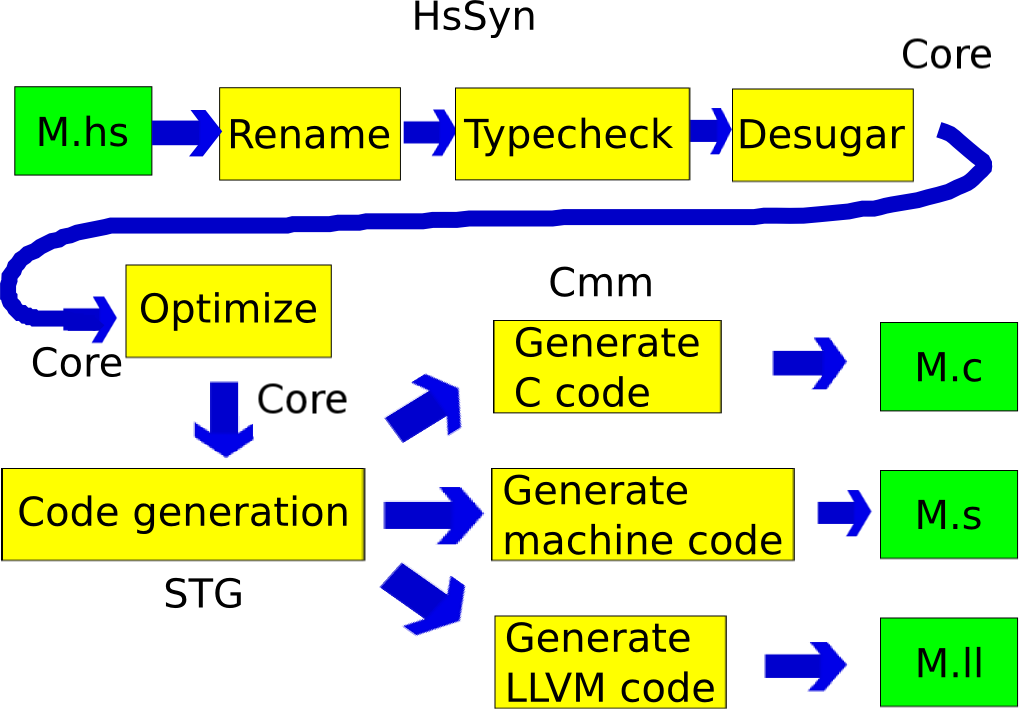
\includegraphics[scale=0.20]{../resources/razvojneEtape.png}
				\end{center}
				\caption{Razvojne etape pravljenja izvršnog k\^{o}da}
				\label{fig:razvojneEtaple}
			\end{figure}
		\end{column}
	\end{columns}
\end{frame}

\section{Frontend}

\begin{frame}{Frontend}
	\begin{itemize}
		\item Parsiranje (eng. \emph{Parser})
		\item Promena imena (eng. \emph{Rename}) 
		\item Provera tipa (eng. \emph{Typecheck})
		\item Prečišćavanje (eng. \emph{Desugaring})
	\end{itemize} 
\end{frame}

\begin{frame}{Parsiranje i promena imena}
	\begin{itemize}
		\item Parsiranje:
		\begin{itemize}
			\item Šabloni (eng. \emph{Pattern})
			\item Infiksni operatori
			\item Poruke o greškama
		\end{itemize}	
	\end{itemize}
	
	\begin{itemize}
		\item Promena imena:
		\begin{itemize}
			\item Zamena \textit{RdrNames} sa \textit{Names}
			\item Analiza zahteva za uzajmno rekurzivne grupe deklaracija
			\item Veliki broj provera grešaka
		\end{itemize}	
	\end{itemize}
	

\end{frame}

\begin{frame}[fragile]{Promena imena}
	
		%\item 	Primer zamene \textit{RdrNames} sa \textit{Names}:
		\begin{block}{Primer zamene \textit{RdrNames} sa \textit{Names}:}
			module $ K $ where
			$ f $ $ x $ = True
			
			module $ N $ where
			import $ K $
			
			module $ M $ where
			import $ N( f ) $ as $ Q $ 
			$f = (f, M.f, Q.f,  \setminus f  -> f) $
		\end{block}

\end{frame}

\begin{frame}{Provera tipa i prečišćavanje}
	\begin{itemize}
	\item Provera tipa:
	\begin{itemize}
		\item Provera programa
		\item Definisanje apstraktne sintakse
		\item Interfejs typechecker-a 
		\item Funkcije tcRnModule i tcRnModuleTcRnM 
	\end{itemize}
	\end{itemize}
	
	\vspace{0.5cm}
	\begin{itemize}
	\item Prečišćavanje: \begin{itemize}
		\item Prevod iz HsSyn tipa u GHC-ov međujezik CoreSyn
	\end{itemize}
	\end{itemize}
\end{frame}

\begin{frame}{Core jezik}
		
	\begin{itemize}
		\item Pravi jednostavan tipizirani lambda račun
		\item Jednostavan lenji funkcionalni jezik Asembler funkcionalnog jezika
	\end{itemize}
	\begin{itemize}
		\item Sastoji od nekoliko elemenata:
	\begin{itemize}
		\item varijable
		\item literali
		\item let
		\item case
		\item lambda apstrakcije
		\item aplikacije
	\end{itemize}
	\end{itemize}
\end{frame}

\section{Middle end}

\begin{frame}{Middle end i umetanje}
	\begin{itemize}
		\item Dodatna optimizacija:
		\begin{itemize}
			\item  umetanje k\^{o}da (eng. \emph{inlining})
			\begin{itemize}
				\item ubrzanje  od 20 – 40\% kod funkcionalnih jezika
				\item ubrzanje od  10 - 15\% kod imperativnih jezika
			\end{itemize}
			\item  eliminacija zajedničkih podizraza (eng. \emph{common subexpression elimination})
		\end{itemize}
	\end{itemize}
\end{frame}

\begin{frame}[fragile]{Umetanje}
		\begin{block}{Samoumetanje (eng. \emph{inlining itself})}
			let $  f = \setminus x -> x*3  $ in $  f (a + b) - c $
			\\$ \implies [inline \hspace{1mm} f] $
			\\let $  f = \setminus x -> x*3  $ in $ (\setminus x -> x*3) (a + b) - c $
		\end{block}
		\begin{block}{Eliminacija mrtvog k\^{o}da (eng. \emph{dead code elimination}) }
			let  $ f = \setminus x -> x*3 $ in $ (\setminus x -> x*3) (a + b) - c $
			\\$ \implies [dead \hspace{1mm} f] $
			\\$ (\setminus x -> x*3) (a + b) - c $
		\end{block}
		\begin{block}{$\beta$  redukcija (eng. \emph{beta reduction})}
		$ (\setminus x -> x*3) (a + b) - c $
		$ \implies [beta] $
		$ (let  \hspace{1mm}  \{ x = a+b \}  \hspace{1mm}  in  \hspace{1mm}  x*3) - c $
		\end{block}
\end{frame}

\begin{frame}[fragile]{Transformacije uslova}

	Razmotrimo, izraz:
	\begin{block}{}
	if (x $ || $ y) then E1 else E2
	\end{block}

	Ovde je $ || $ je operator disjunkcije, definisan sa:
	\begin{block}{}
	$ || $ = $ \setminus $ a b $ \rightarrow $ case a of {True $ \rightarrow $ True; False $ \rightarrow $ b}
	\end{block}

	Jednostavno izvršimo “case-case” transformacije:
	\begin{block}{}
		case (case x of {True $ \rightarrow $ True ; False $ \rightarrow $ y}) of\\
		True $ \rightarrow $ E1\\
		False $ \rightarrow $ E2
	\end{block}
\end{frame}

\begin{frame}[fragile]{Pridruživanje tačaka}
		
		Sada, primenjujući (novu) “case-case” transformaciju, dobijamo:
		\begin{block}{}
			let e1 = E1 ; e2 = E2 \\
			in case x of \\
			True $ \rightarrow $ case True of {True $ \rightarrow $ e1; False $ \rightarrow $ e2} \\
			False $ \rightarrow $ case y of {True $ \rightarrow $ e1; False $ \rightarrow $ e2}
		\end{block}
		
		Dalje vršimo transformaciju “poznatih-konstruktora”
		\begin{block}{}
			let e1 = E1 \\
			in case x of \\
			True $ \rightarrow $ e1 \\
			False $ \rightarrow $ case y of {True $ \rightarrow $ e1; False $ \rightarrow $ E2}
		\end{block}
\end{frame}

\section{Backend}

\begin{frame}{Backend}

	\begin{itemize}
		\item 	Prevođenje \textit{CoreSyn} u \textit{StgSyn (GHC’s intermediate language)}, i to u dve faze:
		\begin{itemize}
			\item CorePrep 
			\begin{itemize}
				\item A-normalna forma (eng. \emph{A-normal form (ANF)}) -  Sabry i Fellisen 1992. godine.
				Na primer:
				\begin{block}{}
					f(g(x),h(y))\\
					let $ v_{0} $ = g(x) in \\
					let $ v_{1} $ = h(y) in  \\
					f($ v_{0}, v_{1} $) 
				\end{block}
				
			\end{itemize} 
			\item CoreToStg
		\end{itemize}
		
		\vspace{0.5cm}
		
		\item STG program se pomoću generatora k\^{o}da pretvara u C-\,-.
	\end{itemize}

\end{frame}

\begin{frame}{GHC k\^{o}d generator}
	
	\begin{itemize}
		\item Ideja:
		
		\begin{itemize}
			\item Problemi sa prevođenjem na C
			\item Podrška za k\^{o}d generatore niskog nivoa
			\item Razvoj jezika srednje-niskog nivoa
		\end{itemize}
	\end{itemize}

	\begin{itemize}
		\item Najznačajniji programi za generisanje izvršnog k\^{o}da::
		
		\begin{itemize}
			\item NGC (eng. \emph{Native Generated Code})
			\item LLVM
			
		\end{itemize}
	\end{itemize}
	
\end{frame}

\begin{frame}[fragile]{LLVM - razlozi implementacije}
	\begin{itemize}
		\item Potreba za pravljenjem kompajlera visokih performansi za generisanje k\^{o}da
		\item GHC proizvodi Haskel programe koji se brzo izračunavaju
		\item Prilagođavanje svake nove verzije LLVM-a postojećoj aplikaciji GHC-a
		\item Uključuje celokupan lanac alata
	\end{itemize}

\end{frame}

\begin{frame}[fragile]{Zaključak}
	\begin{table}[h!]
		\begin{center}
			\caption{Različita vremena generisanja izvršnih k\^{o}dova}
			\begin{tabular}{||c|c|c|c||} \hline
				GHC-6.13 (NCG) & GHC-6.13 (C) & GHC-6.13 (LLVM) & GCC-4.4.3 \\ \hline
				2.876s & 0.576s & 0.516s & 0.335s \\ \hline
			\end{tabular}
			\label{tab:vremena}
		\end{center}
	\end{table}
\end{frame}

\begin{frame}[fragile]{Literatura}
	\begin{itemize}
		\item Edgewall Software. The Glasgow Haskell, Current Status, 2018. on-line: https://ghc.haskell.org/trac/ghc
		\item Stanford University. Why is haskell difficult, 2018. \\on-line: http://www.scs.stanford.edu/11au-cs240h/notes/ghc.html
		\item Simon Marlow (editor). Haskell 2010 Language Report. Haskell community, April 2010
		
		
	\end{itemize}
\end{frame}

\begin{frame}[fragile]{Kraj}
	
	\begin{center}
		Hvala na pažnji! \\
		\vspace{0.5cm}
		Pitanja?
	\end{center}
\end{frame}

\end{document}
